\documentclass[11pt,letterpaper]{article}
\usepackage[lmargin=1in,rmargin=1in,tmargin=1in,bmargin=1in]{geometry}
\usepackage{../style/homework}
\usepackage{../style/commands}
\setbool{quotetype}{false} % True: Side; False: Under
\setbool{hideans}{true} % Student: True; Instructor: False

% -------------------
% Content
% -------------------
\begin{document}

\homework{12: Due 11/05}{Science and everyday life cannot and should not be separated.}{Rosalind Franklin}

% Problem 1
\problem{10} Use the quadratic formula to factor $x^2 - 6x - 3$. Show all your work.

\newpage

% Problem 2
\problem{10} Use the quadratic formula to factor $x^2 - 6x + 10$. Show all your work.

\newpage


% Problem 3
\problem{10} Use the quadratic formula to factor $4x^2 - 8x + 3$. Show all your work.

\newpage


% Problem 4
\problem{10} Find the $x$-intercepts of the quadratic function $y= x^2 - 11x + 30$. Show all your work.

\newpage

% Problem 5
\problem{10} Find the $x$-intercepts of the quadratic function $y= x^2 - 6x + 9$. Show all your work.


\newpage


% Problem 6
\problem{10} Find the $x$-intercepts of the quadratic function $y= 5x^2 - 19x + 12$. Show all your work.


\newpage

% Problem 7
\problem{10} Plot the function $y= x^2 + 2x - 3$. Your plot should include the vertex, axis of symmetry, $y$-intercept, and $x$-intercepts. Show all your work. 
	\[
	\fbox{
	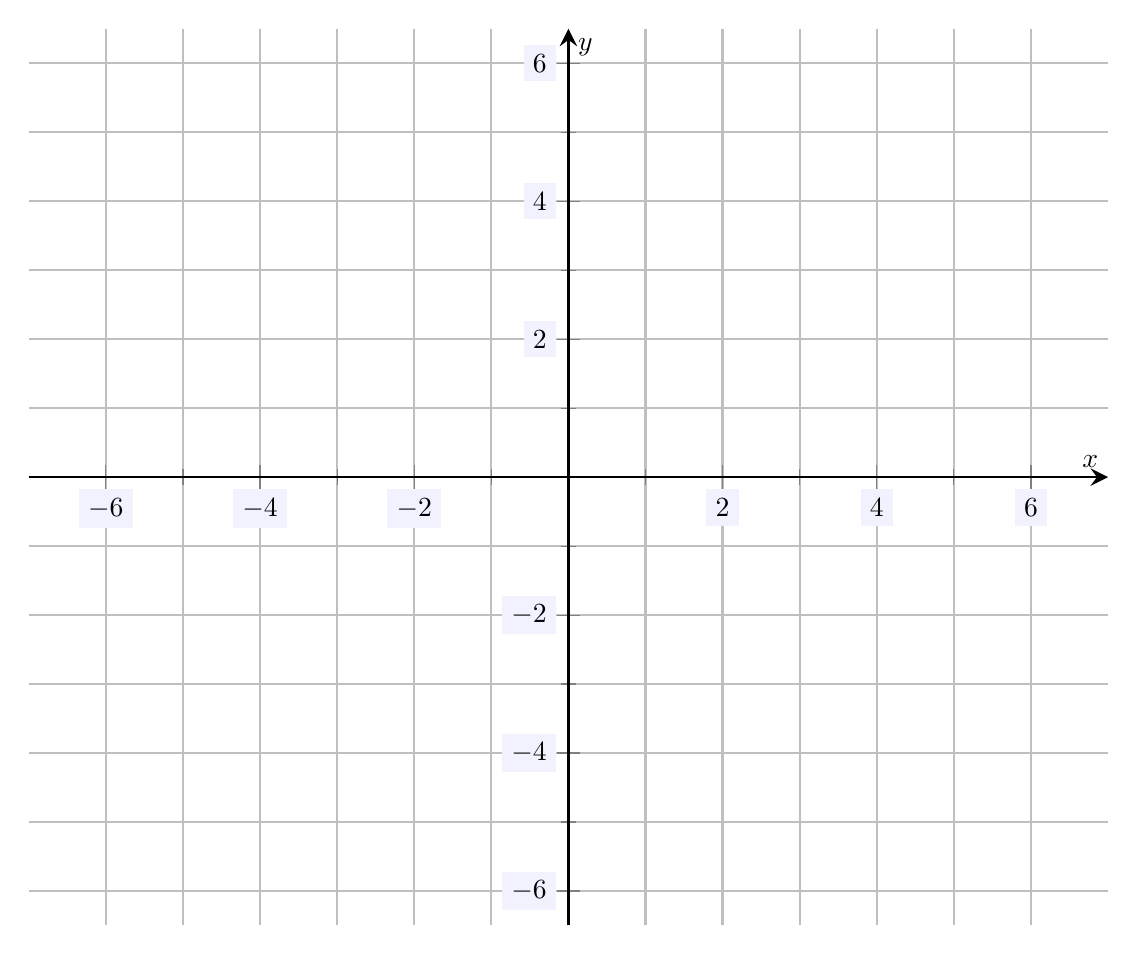
\begin{tikzpicture}[scale=2,every node/.style={scale=0.5}]
	\begin{axis}[
	grid=both,
	axis lines=middle,
	ticklabel style={fill=blue!5!white},
	xmin= -7, xmax=7,
	ymin= -6.5, ymax=6.5,
	xtick={-6,-4,-2,0,2,4,6},
	ytick={-6,-4,-2,0,2,4,6},
	minor tick = {-5,-3,...,5},
	xlabel=\(x\),ylabel=\(y\),
	]
	\end{axis}
	\end{tikzpicture}
	}
	\]






%\printpoints
\end{document}